\documentclass[11pt]{article}
\usepackage{geometry} 
\geometry{a4paper,top=3cm,bottom=3cm,left=2.5cm,right=2.5cm}   
\usepackage{multicol}
\usepackage[english, italian]{babel}
\usepackage{fancyhdr}
\usepackage{fancyvrb}
\usepackage{musicography}
\geometry{centering}
\usepackage{graphicx}
\usepackage{mathpazo} %font
%\usepackage{listings}

%\lstset{size=\tiny}


\pagestyle{fancy}                                 %serve ad inserire la linea sopra e il titolino
\rhead{Lezione 1 "\textit{Programmazione in Faust"}}
\renewcommand{\headrulewidth}{5pt} %grandezza della linea in alto
\renewcommand{\footrulewidth}{1pt}   % grandezza della linea in basso


\begin{document}
\begin{minipage}{0.55\linewidth}
\vspace{0.3cm}
\large{\textbf{Gabriele Petrillo}}\\
\end{minipage}

\vspace{0.3cm}
\begin{minipage}{0.95\linewidth}
\begin{center}
\huge{\textbf{Programmazione in Faust}} \\
\end{center}
\end{minipage}
\vspace*{0.2cm}


%=========ABSTRACT=======================
\begin{center}
\begin{minipage}[c]{14cm}


\textit{L'obiettivo di questa lezione è dare una panoramica ampia del mondo di Faust. Non andremo ancora nei dettagli ma vedremo solo cosa è on grado di fare Faust.}

\end{minipage}
\end{center}
\vspace*{0.2cm}

%=========ARTICOLO========================
\setlength{\columnsep}{3em}

\begin{multicols*}{2}
\parskip=0pt

\textbf{Faust}\\

Faust è un linguaggio di programmazione funzionale per la sintesi del suono e l'elaborazione dell'audio, particolarmente adatto alla progettazione di sintetizzatori, strumenti musicali ed effetti audio. Faust è utilizzato dal vivo per concerti e produzioni artistiche, nella didattica e nella ricerca, in progetti open source e in applicazioni commerciali.
Faust è in grado di scrivere plug-in VST e Audio Unit, realizzare applicazioni Android e IOS, externals per vari linguaggi di computer music come Max, PD, SuperCollider, CSOUND, ChucK e altri ancora. A questo proposito, Faust può essere visto come un'alternativa al C++, ma è molto più semplice e intuitivo da imparare.\\

\textbf{Editor Online}\\

Faust può essere programmato attraverso uno strumento online che non richiede alcuna installazione. Il codice di Faust può essere scritto ed eseguito direttamente in un browser web.

L'editor online di Faust utilizza una tecnologia web all'avanguardia come WebAssembly, e le Web audio API. Per questo motivo, è necessario utilizzare un browser web molto recente che supporti WebAssembly\footnote{WebAssmbly (abbreviato Wasm) è un formato di istruzioni binarie per una virtual-machine stack-based. Wasm è progettato come target portatile per la compilazione di linguaggi di alto livello come \textit{c} e \textit{c++}, consentendo la distribuzione sul web per applicazioni client e server }. Alcune cose avranno bisogno del supporto MIDI e attualmente solo Google Chrome supporta la web midi API, pertanto, si consiglia di utilizzare questo browser.

Apriamo l'editor di Faust\footnote{https://faustide.grame.fr } e scriviamo le prime due righe di codice:

\begin{Verbatim}[fontsize=\footnotesize]

import("stdfaust.lib");
process = + ;

\end{Verbatim}

Queste prime due righe di codice sono molto importanti. La prima importa la libreria standard di Faust, mentre la seconda è la dichiarazione della keyword \textit{process} che rappresenta la funzione main del programma\footnote{In Faust la funzione process equivale alla funzione main dei linguaggi di programmazione \textit{c} o \textit{c++} }.

Quindi, sostituiamo qui la definizione della linea di processo:

\begin{Verbatim}[fontsize=\footnotesize]

import("stdfaust.lib");
process = button("gate") : 
	pm.djembe(60, 0.3, 0.4, 1);

\end{Verbatim}

Button è un interfaccia utente primitiva che genera un segnale pari a 1 ogni volta che viene premuta con il mouse. La grammatica è \textit{button("nome dell'oggetto")}. Adesso tramite i \textit{due punti( : )} possiamo collegare l'uscita del button ad un modello fisico di un djambe \textit{pm.djembe(60,0.3,0.4,1)}, premendo \textit{run} eseguiremo lo script.

In faust le uscite e gli ingressi fisici sono connessi automaticamente, quindi tutti i circuiti sono connessi ai primi ingressi e/o uscite liberi disponibili.\\

\textbf{Primo programma in Faust}\\

Un programma Faust è una serie di istruzioni che terminano con il \textit{punto e virgola ( ; )} è importante non scordare mai il punto e virgola, è l'errore più comune quando si inizia in Faust. L'esempio precedente è composto da due istruzioni: la prima importa l'intera libreria standard di Faust. Una libreria è una collezione di circuiti predefiniti scritti in Faust. Queste collezioni sono organizzate in gerarchie di ambienti che possono essere raggiunti tramite un semplice prefisso. Per esempio, nel codice precedente, \textit{pm.} corrisponde a \textit{physical modelling library}.

La seconda è la nostra \textit{process line} che implementa un semplice djmbe, un modello fisico di una percussione azionata da un bottone. \textit{Button} è un interfaccia utente primitiva\footnote{Gli elementi primitivi sono elementi predefiniti di un linguaggio } che appare come un elemento nell'interfaccia utente grafica. Questo circuito produce un segnale che è zero quando non è premuto, e 1 quando è premuto.

La documentazione di ogni elemento può essere ottenuta semplicemente posizionando il cursore del mouse sopra il nome dell'elemento. Se guardiamo la documentazione di \textit{pm.djembe} possiamo vedere che:

\begin{enumerate}
\item Freq; 
\item Strike position; 
\item Strike sharpness;
\item Gain;
\item Trigger;
\end{enumerate}

Queste rappresentano in ordine gli ingressi del circuito di cui abbiamo definito come parametri i primi quattro e connesso (in maniera automatica visto che era l'unico input vuoto) l'ultimo al \textit{button} tramite il segno dei \textit{due punti ( : )}che collega due circuiti in sequenza. Esiste anche un altra tipologia di notazione che forse rende più chiaro quello che abbiamo programmato:

\begin{Verbatim}[fontsize=\footnotesize]
import("stdfaust.lib");
process = 60, 0.3, 0.4, 1, button("gate") : 
    pm.djembe;
\end{Verbatim}

\begin{center}
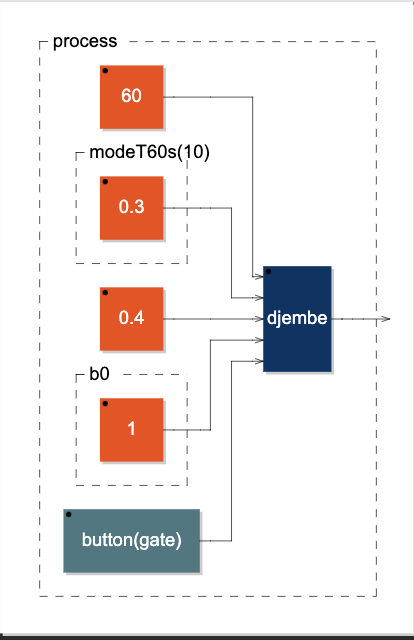
\includegraphics[scale=0.5]{img/01.png}

{\scriptsize \emph{fig.1 }}
\end{center}

\textbf{Aggiungiamo un riverbero}\\

Per aggiungere un riverbero al nostro strumento possiamo utilizzare il riverbero digitale \textit{freeverb} della libreria standard:

\begin{Verbatim}[fontsize=\footnotesize]
import("stdfaust.lib");
process = 60, 0.3, 0.4, 1, button("gate") : 
    pm.djembe : dm.freeverb_demo;
\end{Verbatim}

Tuttavia questo codice produrrà un errore perché \textit{freeverb} ha due input, mentre \textit{djambe} un solo output. Infatti, compilando il codice, verrà visualizzato un errore di questo tipo:

\begin{center}
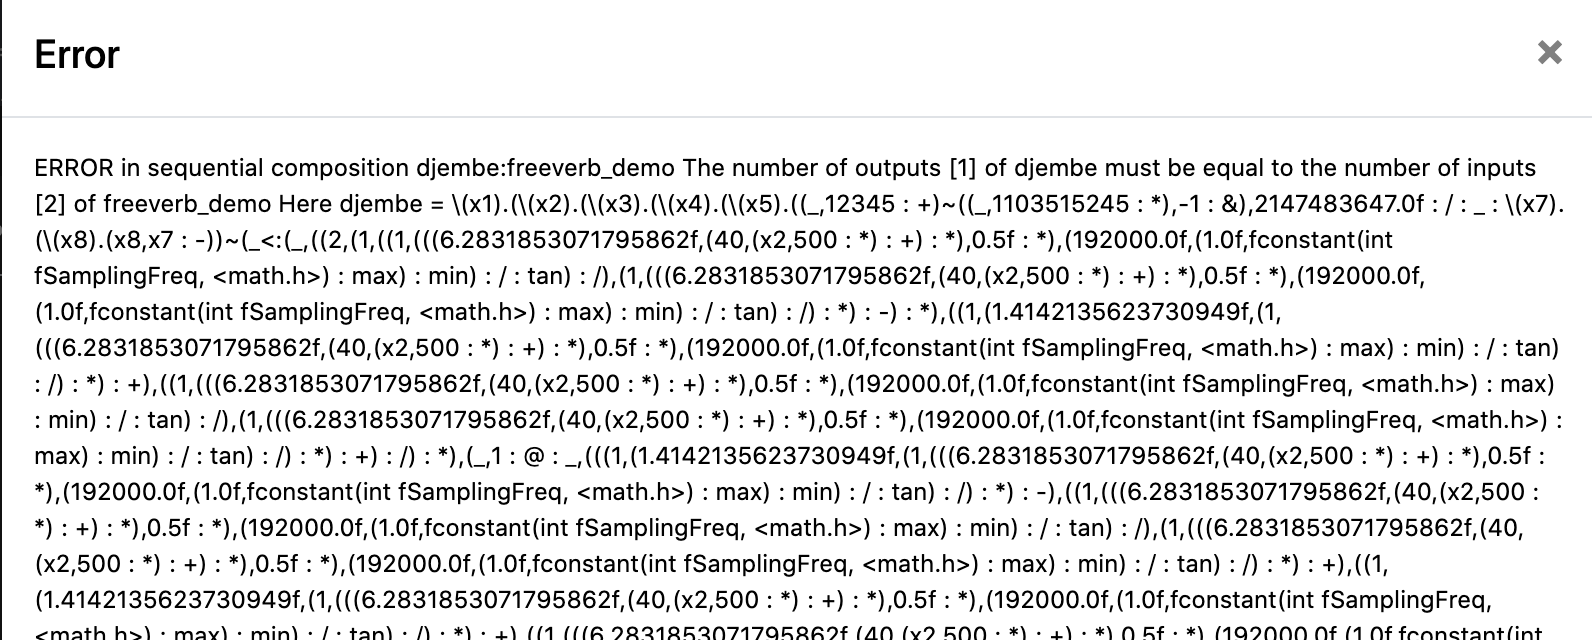
\includegraphics[scale=0.25]{img/02.png}

{\scriptsize \emph{fig.2 }}
\end{center}

\textit{Error in sequential composition, A connected to B, ecc.} vuol dire che il numero di output di A non è lo stesso numero di input di B. Per risolvere il problema dobbiamo utilizzare l'operatore \textit{split composition ( <: )} che divide il segnale in uscita da \textit{djembe} in due segnali:

\begin{Verbatim}[fontsize=\footnotesize]
import("stdfaust.lib");
process = 60, 0.3, 0.4, 1, button("gate") : 
    pm.djembe <: dm.freeverb_demo;
\end{Verbatim}

Compilando il programma possiamo notare molti nuovi elementi nell'interfaccia grafica, questo perché questi elementi sono parte dell'interfaccia grafica di \textit{freeverb}.\\

\textbf{Trigger automatico e costruzione di una mobile App}\\

Possiamo automatizzare la generazione degli impulsi tramite il circuito \textit{ba.pulsen}. Questo dispositivo ha due input, il primo è la dimensione dell'impulso del numero di campioni, nel nostro caso solo un campione. Il secondo è il periodo dell'impulso in campioni. Quindi il periodo è 44100 campioni, dato che la nostra frequenza di campionamento è 44100 Hz avremo un impulso ogni secondo. 

\begin{Verbatim}[fontsize=\footnotesize]
import("stdfaust.lib");
process = button("gate")*ba.pulsen(1,44100) : 
    pm.djembe(60, 0.3, 0.4, 1) <: dm.freeverb_demo;
\end{Verbatim}

È possibile anche inserire altri generatori di impulsi con altri periodi di tempo in modo da creare degli effetti poliritmici.

\begin{Verbatim}[fontsize=\footnotesize]
import("stdfaust.lib");
process = button("gate")*(ba.pulsen(1,44100) + 
    ba.pulsen(1,4410*1.3)) : 
    pm.djembe(60, 0.3, 0.4, 1) <: dm.freeverb_demo;
\end{Verbatim}

Adesso cambiamo nome al nostro programma in alto a sinistra e chiamiamolo \textit{djembe.dsp}.

\begin{center}
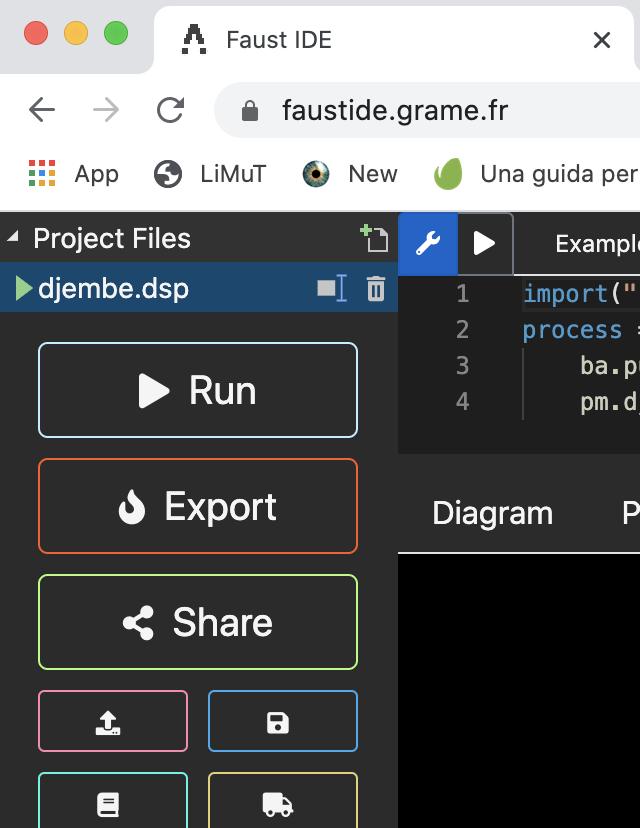
\includegraphics[scale=0.4]{img/03.png}

{\scriptsize \emph{fig.3 }}
\end{center}

Adesso il nostro programma è pronto per essere esportato come un'applicazione Android selezionando \textit{Android platform} e \textit{Android target} nell'export tool dell'editor online. Purtroppo l'editor online non è in grado di generare direttamente delle applicazioni IOS, ma genera un codice che deve essere successivamente compilato sul tuo PC da terminale.\\

\textbf{Oscillatore a dente di sega}\\

L'obiettivo di questa sezione è costruire un semplice generatore di suoni la cui ampiezza sarà controllata soffiando nel microfono del computer. 

Per prima cosa scriviamo un semplice oscillatore a dente di sega con frequenza e gain costanti. Per evitare che il volume sia troppo alto imposteremo il gain a 0.5, tuttavia per poter cambiare facilmente questo parametro in futuro senza modificare la definizione di process possiamo introdurre un nuova variabile chiamata \textit{gain}. Abbiamo due modi di scrivere la nostra linea di process, la prima più intuitiva:

\begin{Verbatim}[fontsize=\footnotesize]
import("stdfaust.lib");
import("stdfaust.lib");
gain = 0.5;
//process = os.sawtooth(440)*gain;
//process = gain, os.sawtooth(440) : *;
\end{Verbatim}

La prima riga di process è una grammatica orientata alla matemica che viene chiamata \textit{infix notation}. La seconda è una scrittura equivalente orientata ai circuiti che consiste nel mettere i dispositivi in parallelo e connetterli in serie ad un moltiplicatore.

Per assegnare un interfaccia grafica al controllo di gain possiamo utilizzare \textit{hslider}, uno slider orizzonatale la cui grammatica è: \textit{hslider("nome", valore di partenza, valore minimo, valore massimo, precisione)}

\begin{Verbatim}[fontsize=\footnotesize]
import("stdfaust.lib");
gain = hslider("gain",0.5, 0, 1, 0.01);
process = os.sawtooth(440)*gain;
\end{Verbatim}

\textbf{Breath control}\\

Per controllare il nostro oscillatore soffiando nel microfono dobbiamo sostituire lo slider con un envelope follower. In Faust il dispositivo per il tracciamento dell'ampiezza è \textit{an.amp\_follower\_ar}. Questo circuito ha tre ingressi:

\begin{enumerate}
\item Durata dell'attacco dell'inviluppo in secondi; 
\item Durata del release in secondi; 
\item Segnale da analizzare;
\end{enumerate}

\begin{Verbatim}[fontsize=\footnotesize]
import("stdfaust.lib");
gain = an.amp_follower_ar(0.02,0.02);
process = gain,os.sawtooth(440):*;
\end{Verbatim}

\textbf{Sintesi additiva}\\

In questa sezione costruiremo un piccolo synth controllato via MIDI. Un piccolo sintetizzatore in sintesi additiva può essere costruito con tre o più oscillatori sinusoidali insieme. Il timbro è determinato dalla relazione dei parametri delle varie armoniche un esempio potrebbe essere il seguente:

\begin{Verbatim}[fontsize=\footnotesize]
import("stdfaust.lib");
process = os.osc(440)*0.5 + 
    os.osc(440*2)*0.25 + 
    os.osc(440*3)*0.125;
\end{Verbatim}

In Faust l'oscillatore sinusoidale è \textit{os.osc}. Ora dobbiamo generalizzare questo codice per ogni frequenza, per farlo dobbiamo introdurre il concetto di parametro. L'esempio precedente può essere riscritto così:

\begin{Verbatim}[fontsize=\footnotesize]
import("stdfaust.lib");
timbro(f) = os.osc(f)*0.5 + 
    os.osc(f*2)*0.25 + 
    os.osc(f*3)*0.125;
process = timbro(440);
\end{Verbatim}

In questo modo possiamo generalizzare questa espressione sostituendo la frequenza con un parametro chiamato \textit{f}. Ora possiamo utilizzare la variabile \textit{timbro} all'interno della linea di process.

Ora se vogliamo controllare il gain e la frequenza del timbro dobbiamo creare due nuove interfacce utente chiamate \textit{frequenza} e \textit{gain} utilizando sempre \textit{hslider}:

\begin{Verbatim}[fontsize=\footnotesize]
import("stdfaust.lib");
freq = hslider("freq", 440, 50, 1000, 0.01);
gain = hslider("gain", 0.5, 0, 1, 0.01);
timbro(f) = os.osc(f)*0.5 + 
    os.osc(f*2)*0.25 + 
    os.osc(f*3)*0.125;
process = gain*timbro(freq);
\end{Verbatim}

\textbf{Sintetizzatore polifonico MIDI}\\

Cerchiamo di capire cosa succede quando premiamo un tasto della nostra tastiera, per prima cosa viene inviato il segnale MIDI \textit{key-on} che contiene due informazioni: il numero del tasto e la velocity. Quando invece lasciamo il tasto viene inviato un messaggio di \textit{key-off} con le stesse informazioni.

In ordine per mappare le informazioni MIDI ai parametri audio del nostro programma dobbiamo rispettare alcune convenzioni per i nomi di questi parametri. Più precisamente devono essere dichiarati tre parametri:

\begin{enumerate}
\item Freq = controllato dal \textit{key number}; 
\item Gain = controllato dalla \textit{velocity}; 
\item Gate = controllato dalla pressione del tasto;
\end{enumerate}

Possiamo quindi testare il programma in due modi differenti: senza polifonia e con il MIDI polifonico. Vediamo un esempio senza nessun device MIDI attaccato implementando un pulsante di gate:

\begin{Verbatim}[fontsize=\footnotesize]
import("stdfaust.lib");
freq = hslider("freq", 440, 50, 1000, 0.01);
gain = hslider("gain", 0.5, 0, 1, 0.01);
gate = button("gate");
timbro(f) = os.osc(f)*0.5 + 
    os.osc(f*2)*0.25 + 
    os.osc(f*3)*0.125;
process = gate*gain*timbro(freq);
\end{Verbatim}

Per il prossimo step dobbiamo necessariamente lavorare sul browser Google Chrome perché è l'unico browser che implementa il supporto MIDI. Ora possiamo utilizzare o una virtual MIDI keyboard come la MidiKeys\footnote{https://flit.github.io/projects/midikeys/} nel Mac o VMPK\footnote{https://vmpk.sourceforge.io} su Linux e Windows. Per controllare un synth monofonico dobbiamo impostare il menù \textit{Poly Voice} a sinistra dell'IDE, a 1, viceversa se lo vogliamo polifonico dobbiamo impostare il numero di voci che vogliamo implementare.

Per evitare i click che si sentono quando eseguiamo una nota dobbiamo inserire un inviluppo collegato all'uscita del gate. In Faust un ADSR è \textit{en.adsr}. Questo dispositivo ha cinque input, rispettivamente:

\begin{enumerate}
\item durata dell'attacco in secondi; 
\item durata del decay in secondi;
\item valore di sustain;
\item durata del release;
\end{enumerate}

\begin{Verbatim}[fontsize=\footnotesize]
import("stdfaust.lib");
freq = hslider("freq", 440, 50, 1000, 0.01);
gain = hslider("gain", 0.5, 0, 1, 0.01);
gate = button("gate") : en.adsr(0.01, 0.01, 0.9, 0.1);
timbro(f) = os.osc(f)*0.5 + 
    os.osc(f*2)*0.25 + 
    os.osc(f*3)*0.125;
process = gain*gate*timbro(freq);
\end{Verbatim}

\textbf{Aggiungiamo un effetto}\\

Se vogliamo aggiungere un effetto ad un synth di questo tipo non dobbiamo aggiungerlo in serie nella riga di process, infatti in questo modo l'effetto sarà duplicato per ogni nota che andremo a suonare e il nostro programma risulterà molto pesante e poco efficiente. Per evitare questo possiamo utilizzare la funzione \textit{effect} che è simile alla funzione \textit{process} e rappresenta un bus dove è indirizzato tutto il segnale in uscita da process. Tuttavia visto che il riverbero \textit{dm.zita\_light} è stereo dobbiamo rendere anche l'otput di process stereo con un'operatore \textit{split}:

\begin{Verbatim}[fontsize=\footnotesize]
import("stdfaust.lib");
freq = hslider("freq", 440, 50, 1000, 0.01);
gain = hslider("gain", 0.5, 0, 1, 0.01);
gate = button("gate") : en.adsr(0.01, 0.01, 0.9, 0.1);
timbro(f) = os.osc(f)*0.5 + 
    os.osc(f*2)*0.25 + 
    os.osc(f*3)*0.125;
process = gain*gate*timbro(freq) <: _,_;
effect = dm.zita_light;
\end{Verbatim}


\end{multicols*}

\end{document}